\documentclass[12pt,a4paper]{article}

% --- Настройка языка и шрифтов для LuaLaTeX ---
\usepackage{fontspec}
\defaultfontfeatures{Ligatures=TeX,Scale=MatchLowercase}

\setmainfont{Times New Roman}

\newfontfamily\cyrillicfont{Times New Roman}

\usepackage{polyglossia}
\setmainlanguage{russian}
\setsansfont{TeX Gyre Heros}
\setmonofont{TeX Gyre Cursor}

\usepackage{graphicx}        					% Графика
\usepackage[protrusion=false]{microtype}       	% Микротипографика
\usepackage{amsmath, amsfonts, amssymb, amsthm}	% Математика
\usepackage{braket} 							% Braket нотация для квантовой механики
\usepackage{unicode-math} 						% Современный пакет для математики в LuaLaTeX
\usepackage{longtable}       					% Таблицы с разрывом страниц
\usepackage{tikz}           					% Рисование
\usepackage[europeanresistors]{circuitikz}		% Рисование электрических схем в европейском стиле
\usepackage{listings}							% Для отображения кода
\usepackage{tabularx}       					% Для таблиц во всю ширину
\usepackage{array}		  						% Для расширенных возможностей таблиц
\usepackage{float}          					% Для точного позиционирования фигур
\usepackage{pgfplots}
\usepackage{caption}
\usepackage{xfp}
\pgfplotsset{compat=1.18}
\usepackage[a4paper,left=20mm,right=20mm,top=20mm,bottom=20mm]{geometry}

\usetikzlibrary{arrows.meta}

% --- Колонтитулы ---
\usepackage{fancyhdr}

\renewcommand{\headrulewidth}{0.4pt}
\renewcommand{\footrulewidth}{0.4pt}
\renewcommand\lstlistingname{Исходный код}

\lstdefinestyle{main}{
	backgroundcolor=\color{gray!8},   
	commentstyle=\color{green!50!black},
	keywordstyle=\color{blue!80!black},
	numberstyle=\small\color{darkgray},
	stringstyle=\rmfamily\color{orange!90!black},
	basicstyle=\ttfamily\small,
	breakatwhitespace=false,         
	breaklines=true,                   
	keepspaces=true,                 
	numbers=left,                    
	numbersep=8pt,                  
	showspaces=false,                
	showstringspaces=false,
	showtabs=false,                  
	tabsize=4
}	

\lstset{style=main}

\newcolumntype{C}{>{\centering\arraybackslash}X}
\renewcommand{\arraystretch}{1.25}

% =========================================================
%         СЛУЖЕБНЫЕ КОМАНДЫ ДЛЯ ВЫЧИСЛЕНИЙ
% =========================================================
\newcommand{\CalcTwo}  [1]{\fpeval{round((#1),2)}}
\newcommand{\CalcThree}[1]{\fpeval{round((#1),3)}}
\newcommand{\CalcFour} [1]{\fpeval{round((#1),4)}}
\newcommand{\CalcFive} [1]{\fpeval{round((#1),5)}}

% ---------------------------------------------------------
% ОБЩИЕ ДАННЫЕ
% ---------------------------------------------------------
\def\VariantN{2}          					 % Номер варианта
\def\StudentName{Анисимов Арсений Сергеевич}  	 % ФИО студента
\def\TeacherName{Устинов Юрий Александрович} % ФИО преподавателя

% Для варианта 1 по методичке:
% Биполярный транзистор: 2N2712
% Полевой транзистор: 2N5558
\def\BJTName{$2$N$1711$}
\def\JFETName{$2$N$5397$}

% ---------------------------------------------------------
% ЗАДАНИЕ 1
% Семейство выходных ВАХ биполярного транзистора
% Таблица 7
% ---------------------------------------------------------
% Далее впишите токи коллектора IК1 ... IК5 для каждого UКЭ
% Столбцы: UКЭ = 0.3, 1, 3, 5, 7, 10 В
% Строка IК1(при IБ1)
\def\IkOneUoThree{\fpeval{478.928 * 10^{-6}}} % IК1 при UКЭ = 0.3 В, мА
\def\IkOneUone   {\fpeval{524.213 * 10^{-6}}} % IК1 при UКЭ = 1 В, мА
\def\IkOneUthree {\fpeval{627.551 * 10^{-6}}} % IК1 при UКЭ = 3 В, мА
\def\IkOneUfive  {\fpeval{730.542 * 10^{-6}}} % IК1 при UКЭ = 5 В, мА
\def\IkOneUseven {\fpeval{833.867 * 10^{-6}}} % IК1 при UКЭ = 7 В, мА
\def\IkOneUten   {\fpeval{988.154 * 10^{-6}}} % IК1 при UКЭ = 10 В, мА

% Строка IК2(при IБ2)
\def\IkTwoUoThree{\fpeval{1.733 * 10^{-3}}} % IК2 при UКЭ = 0.3 В, мА
\def\IkTwoUone   {\fpeval{1.863 * 10^{-3}}} % IК2 при UКЭ = 1 В, мА
\def\IkTwoUthree {\fpeval{2.231 * 10^{-3}}} % IК2 при UКЭ = 3 В, мА
\def\IkTwoUfive  {\fpeval{2.599 * 10^{-3}}} % IК2 при UКЭ = 5 В, мА
\def\IkTwoUseven {\fpeval{2.966 * 10^{-3}}} % IК2 при UКЭ = 7 В, мА
\def\IkTwoUten   {\fpeval{3.518 * 10^{-3}}} % IК2 при UКЭ = 10 В, мА

% Строка IК3(при IБ3)
\def\IkThreeUoThree{\fpeval{3.069 * 10^{-3}}} % IК3 при UКЭ = 0.3 В, мА
\def\IkThreeUone   {\fpeval{3.298 * 10^{-3}}} % IК3 при UКЭ = 1 В, мА
\def\IkThreeUthree {\fpeval{3.951 * 10^{-3}}} % IК3 при UКЭ = 3 В, мА
\def\IkThreeUfive  {\fpeval{4.603 * 10^{-3}}} % IК3 при UКЭ = 5 В, мА
\def\IkThreeUseven {\fpeval{5.255 * 10^{-3}}} % IК3 при UКЭ = 7 В, мА
\def\IkThreeUten   {\fpeval{6.235 * 10^{-3}}} % IК3 при UКЭ = 10 В, мА

% Строка IК4(при IБ4)
\def\IkFourUoThree{\fpeval{4.449 * 10^{-3}}} % IК4 при UКЭ = 0.3 В, мА
\def\IkFourUone   {\fpeval{4.783 * 10^{-3}}} % IК4 при UКЭ = 1 В, мА
\def\IkFourUthree {\fpeval{5.731 * 10^{-3}}} % IК4 при UКЭ = 3 В, мА
\def\IkFourUfive  {\fpeval{6.678 * 10^{-3}}} % IК4 при UКЭ = 5 В, мА
\def\IkFourUseven {\fpeval{7.625 * 10^{-3}}} % IК4 при UКЭ = 7 В, мА
\def\IkFourUten   {\fpeval{9.047 * 10^{-3}}} % IК4 при UКЭ = 10 В, мА

% Строка IК5(при IБ5)
\def\IkFiveUoThree{\fpeval{5.864 * 10^{-3}}} % IК5 при UКЭ = 0.3 В, мА
\def\IkFiveUone   {\fpeval{6.305 * 10^{-3}}} % IК5 при UKЭ = 1 В, мА
\def\IkFiveUthree {\fpeval{7.555 * 10^{-3}}} % IК5 при UКЭ = 3 В, мА
\def\IkFiveUfive  {\fpeval{8.805 * 10^{-3}}} % IК5 при UКЭ = 5 В, мА
\def\IkFiveUseven {\fpeval{10.054 * 10^{-3}}} % IК5 при UКЭ = 7 В, мА
\def\IkFiveUten   {\fpeval{11.929 * 10^{-3}}} % IК5 при UКЭ = 10 В, мА

% ---------------------------------------------------------
% ЗАДАНИЕ 3
% Входная ВАХ биполярного транзистора
% Таблица 8
% ---------------------------------------------------------
% Сначала впишите измеренные токи базы IБ1 ... IБ5 (мкА)
% Они получаются при поочерёдном включении J1 ... J5.
\def\IbOne  {\fpeval{6.106 * 10^{-6}}} % IБ1, А
\def\IbTwo  {\fpeval{19.762 * 10^{-6}}} % IБ2, А
\def\IbThree{\fpeval{33.569 * 10^{-6}}} % IБ3, А
\def\IbFour {\fpeval{47.518 * 10^{-6}}} % IБ4, А
\def\IbFive {\fpeval{61.617 * 10^{-6}}} % IБ5, А
% Впишите измеренные UБЭ при UКЭ = 5 В
% Порядок должен соответствовать IБ1 ... IБ5
\def\UbeOne  {\fpeval{726.249 * 10^{-3}}} % UБЭ1, В
\def\UbeTwo  {\fpeval{760.978 * 10^{-3}}} % UБЭ2, В
\def\UbeThree{\fpeval{776.887 * 10^{-3}}} % UБЭ3, В
\def\UbeFour {\fpeval{787.407 * 10^{-3}}} % UБЭ4, В
\def\UbeFive {\fpeval{795.354 * 10^{-3}}} % UБЭ5, В

% ---------------------------------------------------------
% ЗАДАНИЕ 5
% Стоко-затворная характеристика полевого транзистора
% Таблица 9
% ---------------------------------------------------------
% Впишите точки UЗИ от 0 до Uотс
% Uотс обычно отрицательное
\def\UziOne  {\fpeval{  347 * 10^{-9}}} % первая промежуточная точка UЗИ = 0, В
\def\UziTwo  {\fpeval{  853.273 * 10^{-3}}} % вторая промежуточная точка UЗИ = 0.6, В
\def\UziThree{\fpeval{  1.763}} % третья промежуточная точка UЗИ = 1.2, В
\def\UziFour {\fpeval{  2.398}} % четвёртая промежуточная точка UЗИ = 1.8, В
\def\UziFive {\fpeval{  2.901}} % пятая промежуточная точка UЗИ = 2.4, В
\def\Uots    {\fpeval{  3.47}} % напряжение отсечки Uотс, В

% Впишите соответствующие токи стока IС
\def\IcSat  {\fpeval{  17.314 * 10^{-3}}} % IС.нас при UЗИ = 0, А
\def\IcTwo  {\fpeval{  10.237 * 10^{-3}}} % IС при UЗИ = UziTwo, А
\def\IcThree{\fpeval{  4.715 * 10^{-3}}} % IС при UЗИ = UziThree, А
\def\IcFour {\fpeval{  2.141 * 10^{-3}}} % IС при UЗИ = UziFour, А
\def\IcFive {\fpeval{  756.728 * 10^{-6}}} % IС при UЗИ = UziFive, А
\def\IcCut  {\fpeval{  55.955 * 10^{-6}}} % IС при UЗИ = Uотс, А (обычно близко к 0)

% ---------------------------------------------------------
% ЗАДАНИЕ 7
% Стоковые ВАХ полевого транзистора
% Таблица 10
% ---------------------------------------------------------
% IС при UЗИ = 0
\def\IcUziZeroOne  {\fpeval{7.834 * 10^{-3}}} % при UСИ = 1 В
\def\IcUziZeroTwo  {\fpeval{13.339 * 10^{-3}}} % при UСИ = 2 В
\def\IcUziZeroThree{\fpeval{16.441 * 10^{-3}}} % при UСИ = 3 В
\def\IcUziZeroFour {\fpeval{17.182 * 10^{-3}}} % при UСИ = 4 В
\def\IcUziZeroSix  {\fpeval{17.446 * 10^{-3}}} % при UСИ = 6 В
\def\IcUziZeroEight{\fpeval{17.709 * 10^{-3}}} % при UСИ = 8 В
\def\IcUziZeroTen  {\fpeval{17.973 * 10^{-3}}} % при UСИ = 10 В

% IС при UЗИ = Uотс / 2
\def\IcUziHalfOne  {\fpeval{3.589 * 10^{-3}}} % при UСИ = 1 В
\def\IcUziHalfTwo  {\fpeval{4.744 * 10^{-3}}} % при UСИ = 2 В
\def\IcUziHalfThree{\fpeval{4.781 * 10^{-3}}} % при UСИ = 3 В
\def\IcUziHalfFour {\fpeval{4.818 * 10^{-3}}} % при UСИ = 4 В
\def\IcUziHalfSix  {\fpeval{4.892 * 10^{-3}}} % при UСИ = 6 В
\def\IcUziHalfEight{\fpeval{4.967 * 10^{-3}}} % при UСИ = 8 В
\def\IcUziHalfTen  {\fpeval{5.04 * 10^{-3}}} % при UСИ = 10 В

% =========================================================
%           АВТОМАТИЧЕСКИ ВЫЧИСЛЯЕМЫЕ ВЕЛИЧИНЫ
% =========================================================

% Напряжения источников
\edef\Eone{\CalcTwo{5 + sqrt(\VariantN)}}   % E1 = 5 + sqrt(N)
\edef\Ethree{\CalcTwo{9 + sqrt(\VariantN)}} % E3 = 9 + sqrt(N)

% Uотс / 2
\edef\HalfUots{\CalcFour{\Uots / 2}}

\title{
	МИНОБРНАУКИ РОССИИ

	федеральное государственное автономное образовательное учреждение

	высшего образования

	«Национальный исследовательский университет
	«Московский институт электронной техники»
	\vspace{2em}
}
\author{
}
\date{}

\begin{document}

\maketitle
\thispagestyle{fancy}

\begin{center}
\Large Отчёт по Лабораторной работе $2$\\
по дисциплине «Электроника»\\
«Исследование усилительных элементов»
\end{center}

\begin{center}
\Large Вариант $\VariantN$
\end{center}

\vspace{12em}

\begin{table}[H]
\noindent
\begin{tabular*}{\textwidth}{@{\extracolsep{\fill}} p{0.48\textwidth} p{0.52\textwidth}}
Студент, группа & \StudentName, ЭН-$25$ \\
[0.5em] Руководитель & \TeacherName
\end{tabular*}
\end{table}

\cfoot{Москва 2026}

\pagebreak

\section*{Цель работы}
Исследование биполярных и полевых транзисторов.

\section*{Электрическая схема к $1$-$4$-ому заданиям}

\begin{figure}[H]
\centering
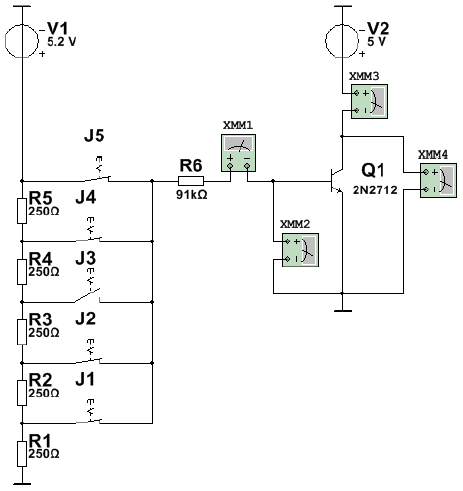
\includegraphics{1experiment.png}
\caption{Схема исследования биполярного транзистора}
\label{1scheme}
\end{figure}

\begin{description}
	\item[V$1$]: источник питания, соглансно $\VariantN$-ому варианту выставлено напряжение $E_1 = 5 + \sqrt{N} = \\ = 5 + \sqrt{\VariantN} = \Eone$ В
	\item[Q$1$]: биполярный транзистор, согласно $\VariantN$-ому варианту выставлен \BJTName
	\item[J$1$]: замыкается $1$-ым для $1$-ого измерения в задании $1$, $3$
	\item[J$2$]: замыкается $2$-ым для $2$-ого измерения в задании $1$, $3$
	\item[J$3$]: замыкается $3$-ым для $3$-ого измерения в задании $1$, $3$
	\item[J$4$]: замыкается $4$-ым для $4$-ого измерения в задании $1$, $3$
	\item[J$5$]: замыкается $5$-ым для $5$-ого измерения в задании $1$, $3$
	\item[XMM$1$]: мультиметр для измерения тока базы $I_\text{Б}$
	\item[XMM$2$]: мультиметр для измерения напряжения базы-эмиттера $U_\text{БЭ}$
	\item[XMM$3$]: мультиметр для измерения тока коллектора $I_\text{К}$
	\item[XMM$4$]: мультиметр для измерения напряжения коллектор-эмиттер $U_\text{КЭ}$
\end{description}

\section{Построение семейства выходных ВАХ биполярного транзистора}
Выставляется  V$2 = 5$ В и поочерёдно замыкаются J$1$ ... J$5$ по одному, измеряется ток базы $I_\text{Б}$
\begin{table}[H]
\centering
\small
\begin{tabularx}{\textwidth}{|p{3cm}|C|C|C|C|C|}
	\hline
	$J$ & $J_1$ & $J_2$ & $J_3$ & $J_4$ & $J_5$ \\
	\hline
	$I_\text{Б}$, мкА & $\fpeval{\IbOne * 10^{6}}$ & $\fpeval{\IbTwo * 10^{6}}$ & $\fpeval{\IbThree * 10^{6}}$ & $\fpeval{\IbFour * 10^{6}}$ & $\fpeval{\IbFive * 10^{6}}$ \\
	\hline
\end{tabularx}
\caption{Токи базы $I_\text{Б}$ при $U_\text{КЭ}=5$ В}
\end{table}

Выставляется V$2 = \{0.3,\ 1,\ 2,\ 3,\ 5,\ 7,\ 10\}$ В и для каждого напряжения $U_\text{КЭ}$ поочерёдно 
замыкаются J$1$ ... J$5$ по одному, измеряется ток коллектора $I_\text{К}$ при каждом токе базы $I_\text{Б}$
\begin{equation*}
I_\text{К} = f(U_\text{КЭ}) \quad \text{при} \quad I_\text{Б} = \text{const}
\end{equation*}

% =========================================================
% ТАБЛИЦА 7
% =========================================================
\begin{table}[H]
\centering
\small
\begin{tabularx}{\textwidth}{|p{3cm}|C|C|C|C|C|C|}
	\hline
	$U_\text{КЭ}$, В & $0.3$ & $1$ & $3$ & $5$ & $7$ & $10$ \\
	\hline
	$I_\text{К1}$ (при $I_\text{Б1}$), мкА & $\fpeval{\IkOneUoThree * 10^{6}}$ & $\fpeval{\IkOneUone * 10^{6}}$ & $\fpeval{\IkOneUthree * 10^{6}}$ & $\fpeval{\IkOneUfive * 10^{6}}$ & $\fpeval{\IkOneUseven * 10^{6}}$ & $\fpeval{\IkOneUten * 10^{6}}$ \\
	\hline
	$I_\text{К2}$ (при $I_\text{Б2}$), мА & $\fpeval{\IkTwoUoThree * 10^{3}}$ & $\fpeval{\IkTwoUone * 10^{3}}$ & $\fpeval{\IkTwoUthree * 10^{3}}$ & $\fpeval{\IkTwoUfive * 10^{3}}$ & $\fpeval{\IkTwoUseven * 10^{3}}$ & $\fpeval{\IkTwoUten * 10^{3}}$ \\
	\hline
	$I_\text{К3}$ (при $I_\text{Б3}$), мА & $\fpeval{\IkThreeUoThree * 10^{3}}$ & $\fpeval{\IkThreeUone * 10^{3}}$ & $\fpeval{\IkThreeUthree * 10^{3}}$ & $\fpeval{\IkThreeUfive * 10^{3}}$ & $\fpeval{\IkThreeUseven * 10^{3}}$ & $\fpeval{\IkThreeUten * 10^{3}}$ \\
	\hline
	$I_\text{К4}$ (при $I_\text{Б4}$), мА & $\fpeval{\IkFourUoThree * 10^{3}}$ & $\fpeval{\IkFourUone * 10^{3}}$ & $\fpeval{\IkFourUthree * 10^{3}}$ & $\fpeval{\IkFourUfive * 10^{3}}$ & $\fpeval{\IkFourUseven * 10^{3}}$ & $\fpeval{\IkFourUten * 10^{3}}$ \\
	\hline
	$I_\text{К5}$ (при $I_\text{Б5}$), мА & $\fpeval{\IkFiveUoThree * 10^{3}}$ & $\fpeval{\IkFiveUone * 10^{3}}$ & $\fpeval{\IkFiveUthree * 10^{3}}$ & $\fpeval{\IkFiveUfive * 10^{3}}$ & $\fpeval{\IkFiveUseven * 10^{3}}$ & $\fpeval{\IkFiveUten * 10^{3}}$ \\
	\hline
\end{tabularx}
\caption{Семейство выходных ВАХ биполярного транзистора}
\end{table}

\section{Расчет коэффициента усиления и выходного сопротивления}
\begin{equation*}
\beta = \frac{\Delta I_\text{К}}{\Delta I_\text{Б}} \quad \text{при} \quad U_\text{КЭ}=5~\text{В} 
\qquad 
r_\text{вых} = \frac{\Delta U_\text{КЭ}}{\Delta I_\text{К}} \quad \text{при} \quad I_\text{Б}=I_\text{Б3}
\end{equation*}

\def\BetaValue{\CalcTwo{(\IkFourUfive - \IkTwoUfive) / (\IbFour - \IbTwo)}}
\def\RoutValue{\CalcTwo{(7 - 3) / (\IkThreeUseven - \IkThreeUthree)}}

Рассчитываем коэффициент усиления 
\begin{equation*}
\beta = \frac{I_\text{К4} - I_\text{К2}}{I_\text{Б4} - I_\text{Б2}} =
\frac{\IkFourUfive - \IkTwoUfive}{\IbFour - \IbTwo} \approx 
\CalcTwo{(\IkFourUfive - \IkTwoUfive) / (\IbFour - \IbTwo)}
\end{equation*}
вокруг точки $I_\text{Б3}$

Рассчитываем выходное сопротивление
\begin{equation*}
r_\text{вых} = \frac{U_\text{КЭ5} - U_\text{КЭ3}}{I_\text{К35} - I_\text{К33}} =
\frac{7 - 3}{\IkThreeUseven - \IkThreeUthree} \approx
\CalcTwo{(7 - 3) / (\IkThreeUseven - \IkThreeUthree)} \text{ Ом}
\end{equation*}
вокруг точки $U_\text{КЭ} = 5$ В

% =========================================================
% ГРАФИК 1
% =========================================================
\begin{figure}[H]
\centering
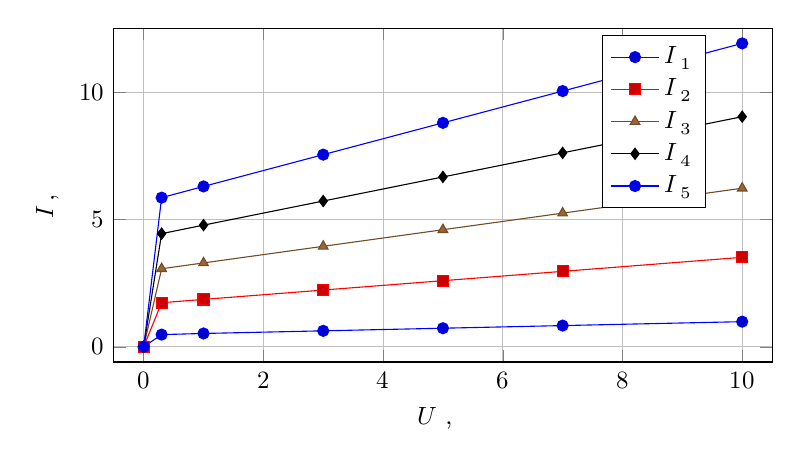
\begin{tikzpicture}
\begin{axis}[
    width=0.82\textwidth,
    height=0.48\textwidth,
    grid=both,
    xlabel={$U_\text{КЭ}$, В},
    ylabel={$I_\text{К}$, мА},
    xmin=\fpeval{-10 * 0.05}, xmax=\fpeval{10 * 1.05}, % Немного больше максимального напряжения для отступа
    ymin=\fpeval{-\IkFiveUten * 10^{3} * 0.05}, ymax=\fpeval{\IkFiveUten * 10^{3} * 1.05}, % Немного больше максимального тока для отступа
    legend style={at={(0.9,0.98)}, anchor=north east, font=\small},
    tick label style={font=\small},
    label style={font=\small}
]
\addplot+[mark=*] coordinates {
    (0,0) (0.3,\fpeval{\IkOneUoThree * 10^{3}}) (1,\fpeval{\IkOneUone * 10^{3}}) (3,\fpeval{\IkOneUthree * 10^{3}})
    (5,\fpeval{\IkOneUfive * 10^{3}}) (7,\fpeval{\IkOneUseven * 10^{3}}) (10,\fpeval{\IkOneUten * 10^{3}})
};
\addplot+[mark=square*] coordinates {
    (0,0) (0.3,\fpeval{\IkTwoUoThree * 10^{3}}) (1,\fpeval{\IkTwoUone * 10^{3}}) (3,\fpeval{\IkTwoUthree * 10^{3}})
    (5,\fpeval{\IkTwoUfive * 10^{3}}) (7,\fpeval{\IkTwoUseven * 10^{3}}) (10,\fpeval{\IkTwoUten * 10^{3}})
};
\addplot+[mark=triangle*] coordinates {
    (0,0) (0.3,\fpeval{\IkThreeUoThree * 10^{3}}) (1,\fpeval{\IkThreeUone * 10^{3}}) (3,\fpeval{\IkThreeUthree * 10^{3}})
    (5,\fpeval{\IkThreeUfive * 10^{3}}) (7,\fpeval{\IkThreeUseven * 10^{3}}) (10,\fpeval{\IkThreeUten * 10^{3}})
};
\addplot+[mark=diamond*] coordinates {
    (0,0) (0.3,\fpeval{\IkFourUoThree * 10^{3}}) (1,\fpeval{\IkFourUone * 10^{3}}) (3,\fpeval{\IkFourUthree * 10^{3}})
    (5,\fpeval{\IkFourUfive * 10^{3}}) (7,\fpeval{\IkFourUseven * 10^{3}}) (10,\fpeval{\IkFourUten * 10^{3}})
};
\addplot+[mark=otimes*] coordinates {
    (0,0) (0.3,\fpeval{\IkFiveUoThree * 10^{3}}) (1,\fpeval{\IkFiveUone * 10^{3}}) (3,\fpeval{\IkFiveUthree * 10^{3}})
    (5,\fpeval{\IkFiveUfive * 10^{3}}) (7,\fpeval{\IkFiveUseven * 10^{3}}) (10,\fpeval{\IkFiveUten * 10^{3}})
};
\legend{$I_\text{Б1}$,$I_\text{Б2}$,$I_\text{Б3}$,$I_\text{Б4}$,$I_\text{Б5}$}
\end{axis}
\end{tikzpicture}
\caption{Семейство выходных ВАХ биполярного транзистора}
\end{figure}

\section{Построение входной ВАХ биполярного транзистора}

Снимаем входную ВАХ биполярного транзистора при $U_\text{КЭ} = 5$ В, поочерёдно замыкая J$1$ ... J$5$ по одному, измеряем $I_\text{Б}$ и $U_\text{БЭ}$ для каждого замыкания
\begin{equation*}
I_\text{Б} = f(U_\text{БЭ}) \quad \text{при} \quad U_\text{КЭ} = 5~\text{В}
\end{equation*}

% =========================================================
% ТАБЛИЦА 8
% =========================================================
\begin{table}[H]
\centering
\small
\begin{tabularx}{\textwidth}{|C|C|C|C|C|C|}
	\hline
	$J$ & $J_1$ & $J_2$ & $J_3$ & $J_4$ & $J_5$ \\
	\hline
	$I_\text{Б}$, мкА & $\fpeval{\IbOne * 10^{6}}$ & $\fpeval{\IbTwo * 10^{6}}$ & $\fpeval{\IbThree * 10^{6}}$ & $\fpeval{\IbFour * 10^{6}}$ & $\fpeval{\IbFive * 10^{6}}$ \\
	\hline
	$U_\text{БЭ}$, мВ & $\fpeval{\UbeOne * 10^{3}}$ & $\fpeval{\UbeTwo * 10^{3}}$ & $\fpeval{\UbeThree * 10^{3}}$ & $\fpeval{\UbeFour * 10^{3}}$ & $\fpeval{\UbeFive * 10^{3}}$ \\
	\hline
\end{tabularx}
\caption{Входная ВАХ биполярного транзистора при $U_\text{КЭ}=5$ В}
\end{table}

\section{Расчет входного сопротивления}

\begin{equation*}
r_\text{вх} = \frac{\Delta U_\text{БЭ}}{\Delta I_\text{Б}} \quad \text{при} \quad I_\text{Б}=I_\text{Б3}
\end{equation*}

\def\RinValue{\CalcTwo{(\UbeFour - \UbeTwo) / (\IbFour - \IbTwo)}}

Рассчитываем входное сопротивление
\begin{equation*}
r_\text{вх} = \frac{U_\text{БЭ4} - U_\text{БЭ2}}{I_\text{Б4} - I_\text{Б2}} =
\frac{\UbeFour - \UbeTwo}{\IbFour - \IbTwo} \approx
\CalcTwo{(\UbeFour - \UbeTwo) / (\IbFour - \IbTwo)} \text{ Ом}
\end{equation*}
вокруг точки $I_\text{Б3}$

% =========================================================
% ГРАФИК 2
% =========================================================
\begin{figure}[H]
\centering
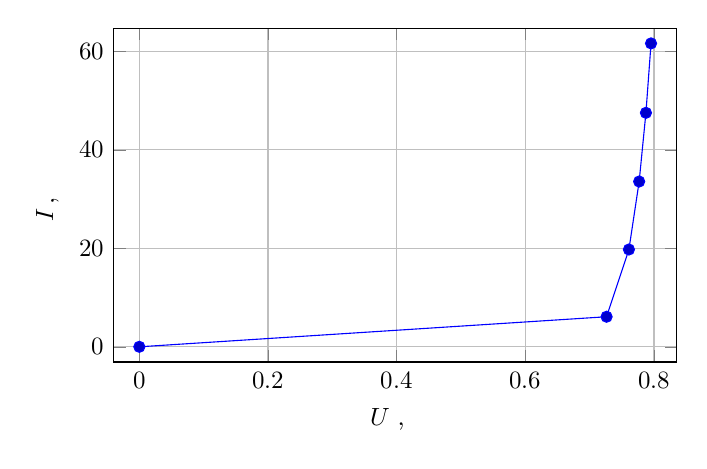
\begin{tikzpicture}
\begin{axis}[
    width=0.72\textwidth,
    height=0.48\textwidth,
    grid=both,
    xlabel={$U_\text{БЭ}$, В},
    ylabel={$I_\text{Б}$, мкА},
	xmin=\fpeval{-\UbeFive * 0.05}, xmax=\fpeval{\UbeFive * 1.05}, % Немного больше максимального напряжения для отступа
    ymin=\fpeval{-\IbFive * 10^{6} * 0.05}, ymax=\fpeval{\IbFive * 10^{6} * 1.05}, % Немного больше максимального тока для отступа
    tick label style={font=\small},
    label style={font=\small}
]
\addplot+[mark=*] coordinates {
	(0,0)
    (\UbeOne,\fpeval{\IbOne * 10^{6}})
    (\UbeTwo,\fpeval{\IbTwo * 10^{6}})
    (\UbeThree,\fpeval{\IbThree * 10^{6}})
    (\UbeFour,\fpeval{\IbFour * 10^{6}})
    (\UbeFive,\fpeval{\IbFive * 10^{6}})
};
\end{axis}
\end{tikzpicture}
\caption{Входная ВАХ биполярного транзистора}
\end{figure}

\section*{Электрическая схема к $5$-$8$-ому заданиям}

\begin{figure}[H]
\centering
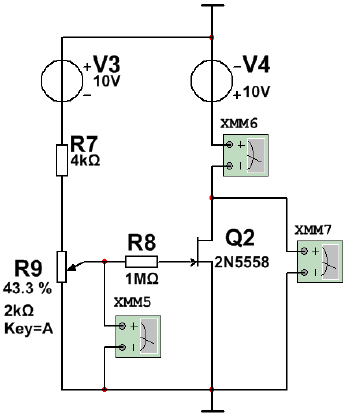
\includegraphics{2experiment.png}
\caption{Схема исследования полевого транзистора}
\end{figure}

\begin{description}
	\item[V$3$]: источник питания, соглансно $\VariantN$-ому варианту выставлено напряжение $E_3 = 9 + \sqrt{N} = \\ = 9 + \sqrt{\VariantN} = \Ethree$ В
	\item[Q$2$]: полевой транзистор, согласно $\VariantN$-ому варианту выставлен \JFETName
	\item[R$9$]: потенциометр, сопротивление $R_9 = 2$ кОм, используется в заданиях $5$, $7$ 
	\item[XMM$5$]: мультиметр для измерения напряжения затвор-исток $U_\text{ЗИ}$
	\item[XMM$6$]: мультиметр для измерения тока стока $I_\text{С}$
	\item[XMM$7$]: мультиметр для измерения напряжения сток-исток $U_\text{СИ}$
\end{description}

\section{Построение стоко-затворной характеристики полевого транзистора}

С помощью потенциометра R$9$ выставляем $U_\text{ЗИ}$ от $\approx 0$ до $U_\text{отс}$ ($I_\text{С.нас} 
\approx 0$) и измеряем $I_\text{С}$ при $U_\text{СИ} = 5$ В
\begin{equation*}
I_\text{С} = f(U_\text{ЗИ}) \quad \text{при} \quad U_\text{СИ} = 5~\text{В}
\end{equation*}

% =========================================================
% ТАБЛИЦА 9
% =========================================================
\begin{table}[H]
\centering
\small
\begin{tabularx}{\textwidth}{|p{1.1cm}|p{2.5cm}|p{2.3cm}|C|C|p{2.3cm}|p{3.0cm}|}
	\hline
	$U_\text{ЗИ}$, В & \centering $\fpeval{\UziOne * 10^{9}} \cdot 10^{-9}$ & $\fpeval{\UziTwo * 10^{3}} \cdot 10^{-3}$ & $\fpeval{\UziThree}$ & \centering $\fpeval{\UziFour}$ & \centering $\fpeval{\UziFive}$ & $U_\text{отс}=\fpeval{\Uots}$ \\
	\hline
	$I_\text{С}$, мА & \centering $I_\text{C.нас} = \fpeval{\IcSat * 10^{3}}$ & \centering $\fpeval{\IcTwo * 10^{3}}$ & $\fpeval{\IcThree * 10^{3}}$ & $\fpeval{\IcFour * 10^{3}}$ & $\fpeval{\IcFive * 10^{6}} \cdot 10^{-3}$ & $I_\text{С}=\fpeval{\IcCut * 10^{6}} \cdot 10^{-3}$ \\
	\hline
\end{tabularx}
\caption{Стоко-затворная характеристика полевого транзистора}
\end{table}

% =========================================================
% ГРАФИК 3
% =========================================================
\begin{figure}[H]
\centering
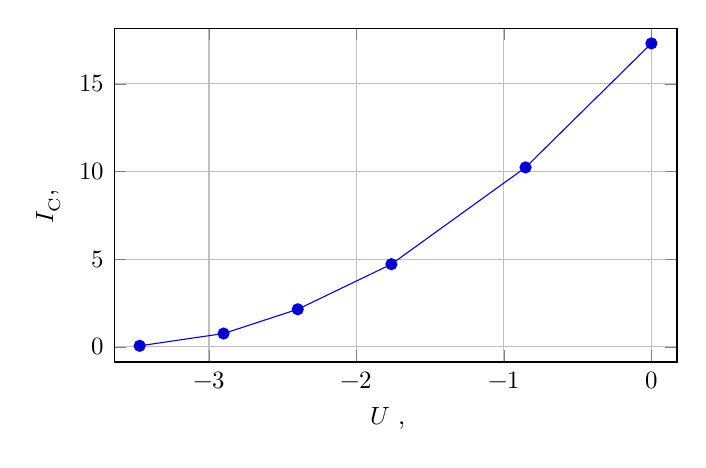
\begin{tikzpicture}
\begin{axis}[
    width=0.72\textwidth,
    height=0.48\textwidth,
    grid=both,
    xlabel={$U_\text{ЗИ}$, В},
    ylabel={$I_\text{C}$, мА},
	xmin=\fpeval{-\Uots * 1.05}, xmax=\fpeval{\Uots * 0.05}, % Немного больше максимального напряжения для отступа
	ymin=\fpeval{-\IcSat * 10^{3} * 0.05}, ymax=\fpeval{\IcSat * 10^{3} * 1.05}, % Немного больше максимального тока для отступа
    tick label style={font=\small},
    label style={font=\small}
]
\addplot+[mark=*] coordinates {
	(\fpeval{-\UziOne},\fpeval{\IcSat * 10^{3}})
	(\fpeval{-\UziTwo},\fpeval{\IcTwo * 10^{3}})
	(\fpeval{-\UziThree},\fpeval{\IcThree * 10^{3}})
	(\fpeval{-\UziFour},\fpeval{\IcFour * 10^{3}})
	(\fpeval{-\UziFive},\fpeval{\IcFive * 10^{3}})
	(\fpeval{-\Uots},\fpeval{\IcCut * 10^{3}})
};
\end{axis}
\end{tikzpicture}
\caption{Стоко-затворная характеристика полевого транзистора}
\end{figure}

\section{Расчёт крутизны}

\begin{equation*}
S = \frac{\Delta I_\text{С}}{\Delta U_\text{ЗИ}}
\end{equation*}

\def\SminValue{\CalcTwo{abs(\IcCut - \IcFive) / (\Uots - \UziFive) * 10^{3}}}
\def\SmaxValue{\CalcTwo{abs(\IcTwo - \IcSat) / (\UziTwo - \UziOne) * 10^{3}}}

Рассчитываем минимальную крутизну
\begin{equation*}
	S_\text{min} = \frac{\left|I_\text{С6} - I_\text{С5}\right|}{U_\text{ЗИ6} - U_\text{ЗИ5}} =
	\frac{\left|\fpeval{\IcCut * 10^{3}} - \fpeval{\IcFive * 10^{3}}\right|}{\fpeval{\Uots} - \fpeval{\UziFive}} \approx
	\CalcTwo{abs(\IcCut - \IcFive) / (\Uots - \UziFive) * 10^{3}} \text{ мА/В}
\end{equation*}
при минимальном токе стока

Рассчитываем максимальную крутизну
\begin{equation*}
	S_\text{max} = \frac{\left|I_\text{С2} - I_\text{С1}\right|}{U_\text{ЗИ2} - U_\text{ЗИ1}} =
	\frac{\left|\fpeval{\IcTwo * 10^{3}} - \fpeval{\IcSat * 10^{3}}\right|}{\fpeval{\UziTwo} - \fpeval{\UziOne}} \approx
	\CalcTwo{abs(\IcTwo - \IcSat) / (\UziTwo - \UziOne) * 10^{3}} \text{ мА/В}
\end{equation*}
при максимальном токе стока

\section{Построение стоковой ВАХ полевого транзистора}

Фиксируем $U_\text{ЗИ}=0$ В и $U_\text{ЗИ}=U_\text{отс}/2=\fpeval{\HalfUots}$ В, и измеряем $I_\text{С}$ при $U_\text{СИ} = \{1,\ 2,\ 3,\ 4,\ \\6,\ 8,\ 10\}$ В
\begin{equation*}
I_\text{С} = f(U_\text{СИ}) \quad \text{при} \quad U_\text{ЗИ} = 0~\text{В} \quad \text{и} \quad U_\text{ЗИ} = U_\text{отс}/2
\end{equation*}

% =========================================================
% ТАБЛИЦА 10
% =========================================================
\begin{table}[H]
\centering
\small
\begin{tabularx}{\textwidth}{|p{4cm}|C|C|C|C|C|C|C|}
	\hline
	$U_\text{СИ}$, В & $1$ & $2$ & $3$ & $4$ & $6$ & $8$ & $10$ \\
	\hline
	$I_\text{С}$ при $U_\text{ЗИ}=0$, мА &
	$\fpeval{\IcUziZeroOne * 10^{3}}$ & $\fpeval{\IcUziZeroTwo * 10^{3}}$ & $\fpeval{\IcUziZeroThree * 10^{3}}$ & $\fpeval{\IcUziZeroFour * 10^{3}}$ &
	$\fpeval{\IcUziZeroSix * 10^{3}}$ & $\fpeval{\IcUziZeroEight * 10^{3}}$ & $\fpeval{\IcUziZeroTen * 10^{3}}$ \\
	\hline
	$I_\text{С}$ при $U_\text{ЗИ}=U_\text{отс}/2$, мА &
	$\fpeval{\IcUziHalfOne * 10^{3}}$ & $\fpeval{\IcUziHalfTwo * 10^{3}}$ & $\fpeval{\IcUziHalfThree * 10^{3}}$ & $\fpeval{\IcUziHalfFour * 10^{3}}$ &
	$\fpeval{\IcUziHalfSix * 10^{3}}$ & $\fpeval{\IcUziHalfEight * 10^{3}}$ & $\fpeval{\IcUziHalfTen * 10^{3}}$ \\
	\hline
\end{tabularx}
\caption{Стоковые ВАХ полевого транзистора}
\end{table}

% =========================================================
% ГРАФИК 4
% =========================================================
\begin{figure}[H]
\centering
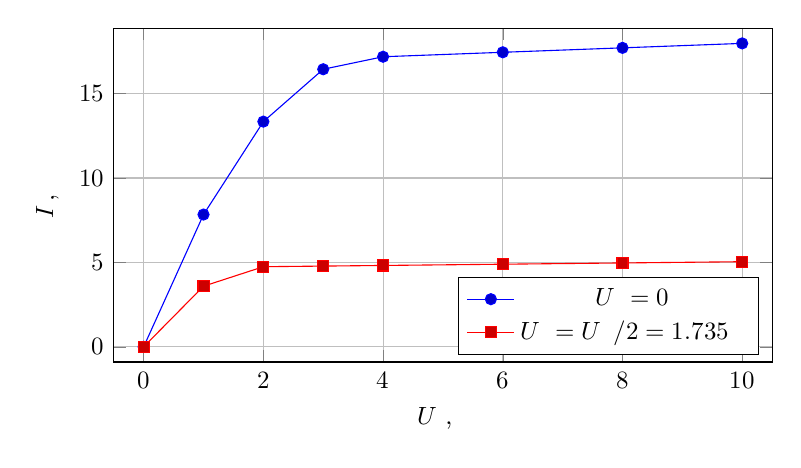
\begin{tikzpicture}
\begin{axis}[
    width=0.82\textwidth,
    height=0.48\textwidth,
    grid=both,
    xlabel={$U_\text{СИ}$, В},
    ylabel={$I_\text{С}$, мА},
    xmin=\fpeval{-10 * 0.05}, xmax=\fpeval{10 * 1.05}, % Немного больше максимального напряжения для отступа
    ymin=\fpeval{-\IcUziZeroTen * 10^{3} * 0.05}, ymax=\fpeval{\IcUziZeroTen * 10^{3} * 1.05}, % Немного больше максимального тока для отступа
    legend style={at={(0.98,0.02)}, anchor=south east, font=\small},
    tick label style={font=\small},
    label style={font=\small}
]
\addplot+[mark=*] coordinates {
	(0,0)
    (1,\fpeval{\IcUziZeroOne * 10^{3}})
    (2,\fpeval{\IcUziZeroTwo * 10^{3}})
    (3,\fpeval{\IcUziZeroThree * 10^{3}})
    (4,\fpeval{\IcUziZeroFour * 10^{3}})
    (6,\fpeval{\IcUziZeroSix * 10^{3}})
    (8,\fpeval{\IcUziZeroEight * 10^{3}})
    (10,\fpeval{\IcUziZeroTen * 10^{3}})
};
\addplot+[mark=square*] coordinates {
	(0,0)
    (1,\fpeval{\IcUziHalfOne * 10^{3}})
    (2,\fpeval{\IcUziHalfTwo * 10^{3}})
    (3,\fpeval{\IcUziHalfThree * 10^{3}})
    (4,\fpeval{\IcUziHalfFour * 10^{3}})
    (6,\fpeval{\IcUziHalfSix * 10^{3}})
    (8,\fpeval{\IcUziHalfEight * 10^{3}})
    (10,\fpeval{\IcUziHalfTen * 10^{3}})
};
\legend{$U_\text{ЗИ}=0$,$U_\text{ЗИ}=U_\text{отс}/2 = \HalfUots$ В}
\end{axis}
\end{tikzpicture}
\caption{Стоковые ВАХ полевого транзистора}
\end{figure}

\section*{Выводы}

В ходе выполнения лабораторной работы были исследованы биполярный и полевой транзисторы.

Для биполярного транзистора были сняты и построены семейство выходных ВАХ и входная ВАХ, 
а также рассчитаны коэффициент усиления по току и дифференциальные выходное и входное сопротивления. 

Полученые характеристики для биполярного транзистора:
\begin{equation*}
\beta \approx \BetaValue, \qquad
r_\text{вых} \approx \RoutValue \ \text{Ом}, \qquad
r_\text{вх} \approx \RinValue \ \text{Ом}.
\end{equation*}

Для полевого транзистора была снята стоко-затворная характеристика, определены ток насыщения стока и 
напряжение отсечки, а также построены стоковые ВАХ при $U_\text{ЗИ}=0$ и $U_\text{ЗИ}=U_\text{отс}/2 = 
\HalfUots$. 

Полученые характеристики для полевого транзистора:
\begin{equation*}
U_\text{отс} = \Uots \ \text{В}, \qquad
S_\text{min} \approx \SminValue \ \text{мА/В}, \qquad
S_\text{max} \approx \SmaxValue \ \text{мА/В}.
\end{equation*}

Построенные характеристики подтверждают усилительные свойства исследованных приборов и позволяют 
оценить их основные параметры в рабочем режиме.

\end{document}